% -*- TeX-master: "sbml-level-3-version-1-core"; fill-column: 66 -*-
% $Id$
% $HeadURL$
% ----------------------------------------------------------------

\section{Preliminary definitions and principles}
\label{sec:general}

This section covers certain concepts and constructs that are used
repeatedly in the rest of SBML \thisL.


\subsection{Primitive data types}
\label{sec:primitive-types}

Most primitive types in SBML are taken from the data types defined
in \xmlschemaone~\citep{biron:2000,fallside:2000,thompson:2000}.
A few other primitive types are defined by SBML itself.  What
follows is a summary of the XML Schema types and the definitions
of the SBML-specific types.  Note that while we have tried to
provide accurate and complete summaries of the XML Schema types,
the following should not be taken to be normative definitions of
these types.  Readers should consult the \xmlschemaone
specification for the normative definitions of the XML data types
used by SBML.


\subsubsection{Type \primtype{string}}
\label{sec:string}

The \xmlschemaone type \primtype{string} is used to represent
finite-length strings of characters.  The characters permitted to
appear in XML Schema \primtype{string} include all Unicode
characters~\citep{unicode:1996} except for two delimiter
characters, 0xFFFE and 0xFFFF~\citep{biron:2000}.  In addition,
the following quoting rules specified by XML for character
data~\citep{bray:2000} must be obeyed:
\begin{itemize}

\item The ampersand (\texttt{\&}) character must be escaped using
  the entity \texttt{\&amp;}.

\item The apostrophe (\texttt{'}) and quotation mark (\texttt{"})
  characters must be escaped using the entities \texttt{\&apos;}
  and \texttt{\&quot;}, respectively, when those characters are
  used to delimit a string attribute value.

\end{itemize}
Other XML built-in character or entity references, e.g.,
\texttt{\&lt;} and \texttt{\&x1A;}, are permitted in strings.


\subsubsection{Type \primtype{boolean}}
\label{sec:boolean}

The \xmlschemaone type \primtype{boolean} is used as the data type
for SBML object attributes that represent binary true/false values.
\xmlschemaone defines the possible literal values of
\primtype{boolean} as the following: \val{true}, \val{false},
\val{1}, and \val{0}.  The value \val{1} maps to \val{true} and
the value \val{0} maps to \val{false}.

Note that there is a discrepancy between the value spaces of type
\primtype{boolean} as defined by \xmlschemaone and \mathml: the
latter uses only \val{true} and \val{false} to represent boolean
values and \val{0} and \val{1} are interpreted as numbers.
Software tools should take care to not to use \val{0} and \val{1}
as boolean values in \mathml expressions.  See further discussion
in Section~\ref{sec:handling-booleans}.


\subsubsection{Type \primtype{int}}
\label{sec:integer}

The \xmlschemaone type \primtype{int} is used to represent decimal
integer numbers in SBML.  The literal representation of an
\primtype{int} is a finite-length sequence of decimal digit
characters with an optional leading sign (\val{+} or \val{-}).  If
the sign is omitted, \val{+} is assumed.  The value space of
\primtype{int} is the same as a standard 32-bit signed integer in
programming languages such as C, \ie 2147483647 to $-2147483648$.


\subsubsection{Type \primtype{positiveInteger}}
\label{sec:positiveinteger}

The \xmlschemaone type \primtype{positiveInteger} is used to
represent nonzero, nonnegative, decimal integers: \ie 1, 2, 3,
\ldots.  The literal representation of an integer is a
finite-length sequence of decimal digit characters, optionally
preceded by a positive sign (``\token{+}'').  There is no
restriction on the absolute size of \primtype{positiveInteger}
values in XML Schema; however, the only situations where this type
is used in SBML involve very low-numbered integers.  Consequently,
applications may safely treat \primtype{positiveInteger} as
unsigned 32-bit integers.


\subsubsection{Type \primtype{double}}
\label{sec:double}

The \xmlschemaone type \primtype{double} is the data type of
floating point numerical quantities in SBML.  It is restricted to IEEE
double-precision 64-bit floating point type IEEE 754-1985.  The
value space of \primtype{double} consists of (a) the numerical
values $m \cdot 2^x$, where $m$ is an integer whose absolute
value is less than $2^{53}$, and $x$ is an integer between -1075
and 970, inclusive, (b) the special value positive infinity
(\token{INF}), (c) the special value negative infinity
(\token{-INF}), and (d) the special value not-a-number
(\token{NaN}).  The order relation on the values is the following:
$x < y$ if and only if $y - x$ is positive for values of $x$ and
$y$ in the value space of \primtype{double}.  Positive infinity is
greater than all other values other than \token{NaN}.  \token{NaN}
is equal to itself but is neither greater nor less than any other
value in the value space.  (Software implementors should consult
the \xmlschemaone definition of \primtype{double} for additional
details about equality and relationships to IEEE 754-1985.)

The general form of \primtype{double} numbers is
  \val{$x$e$y$}, where $x$ is a decimal number (the mantissa),
  \val{e} is a separator character, and $y$ is an
  exponent; the meaning of this is ``$x$ multiplied by 10 raised
  to the power of $y$'', i.e., $x \cdot 10^y$.  More
precisely, a \primtype{double} value consists of a mantissa with
an optional leading sign (\val{+} or \val{-}), optionally followed
by the character \token{E} or \token{e} followed by an integer
(the exponent).  The mantissa must be a decimal number: an integer
optionally followed by a period (\token{.})\ optionally followed
by another integer.  If the leading sign is omitted, \val{+} is
assumed.  An omitted \token{E} or \token{e} and exponent means
that a value of 0 is assumed for the exponent.  If the \token{E}
or \token{e} is present, it must be followed by an integer or an
error results.  The integer acting as an exponent must consist of
a decimal number optionally preceded by a leading sign (\val{+} or
\val{-}).  If the sign is omitted, \val{+} is assumed.  The
following are examples of legal literal \primtype{double} values:
\begin{center}
\begin{tabular}{llllllllllll}
\token{-1E4}, & \token{+4}, & \token{234.234e3}, & \token{6.02E-23}, 
& \token{0.3e+11}, & \token{2}, & \token{0}, & \token{-0}, 
& \token{INF}, & \token{-INF}, & \token{NaN}
\end{tabular}
\end{center}

As described in Section~\ref{sec:formulas}, SBML uses a subset of
the \mathmltwo standard~\citep{w3c:2000b} for expressing
mathematical formulas in XML.  This is done by stipulating that
the MathML language be used whenever a mathematical formula must
be written into an SBML model.  Doing this, however, requires
facing two problems: first, the syntax of numbers in scientific
notation (``e-notation'') is different in MathML from that just
described for \token{double}, and second, the value space of
integers and floating-point numbers in MathML is not defined in
the same way as in \xmlschemaone.  We elaborate on these issues in
Section~\ref{sec:cn-token}; here we summarize the solution taken
in SBML.  First, within MathML, the mantissa and exponent of
numbers in ``e-notation'' format must be separated by one
\texttt{<sep/>} element.  This leads to numbers of the form
\texttt{<cn type="e-notation"> 2 <sep/> -5 </cn>}.  Second, SBML
stipulates that the representation of numbers in MathML
expressions obey the same restrictions on values as defined for
types \primtype{double} and \primtype{int}
(Section~\ref{sec:integer}).


\subsubsection{Type \primtype{ID}}
\label{sec:id}

The \xmlschemaone type \primtype{ID} is identical to the XML 1.0
type \primtype{ID}.  The literal representation of this type
consists of strings of characters restricted as summarized in
Figure~\ref{fig:id}.

% For a good summary of CombiningChar and Extender see
% http://xsd.stylusstudio.com/2003Sep/post05008.htm


\begin{figure}[htb]
  \ttfamily
  \small
  \centering
  \vspace*{-1ex}
  \begin{edtable}{tabular}{lll}
    NameChar & ::= & letter | digit | '.' | '-' | '\_' | ':' | CombiningChar | Extender\\
    ID       & ::= & ( letter | '\_' | ':' ) NameChar*
  \end{edtable}
  \vspace*{-3pt}
  \caption{Type \primtype{ID}
    expressed in the variant of BNF used by the XML 1.0
    specification~\protect\citep{bray:2004}.  The characters
    \texttt{(} and \texttt{)} are used for grouping, the character
    \texttt{*} indicates ``zero or more times'', and the character
    \texttt{|} indicates ``or''.  The production \token{letter}
    consists of the basic upper and lower case alphabetic
    characters of the Latin alphabet along with a large number of
    related characters defined by Unicode~2.0; similarly, the
    production \token{digit} consists of the numerals
    \texttt{0..9} along with related Unicode~2.0 characters.  The
    \token{CombiningChar} production is a list of characters that
    add such things as accents to the preceding character. (For
    example, the Unicode character \token{\#x030A} when combined
    with `a' produces `\aa'.)  The \token{Extender} production is
    a list of characters that extend the shape of the preceding
    character.  Please consult the XML~1.0
    specification~\protect\citep{bray:2004} for the complete
    definitions of \token{letter}, \token{digit},
    \token{CombiningChar}, and \token{Extender}.}
  \label{fig:id}
\end{figure}

In SBML, type \primtype{ID} is the data type of the \token{metaid}
attribute on \SBase, described in
Section~\ref{sec:sbase}.  An important aspect of \primtype{ID} is
the XML requirement that a given value of \primtype{ID} must be
unique throughout an XML document.  All data values of type
\primtype{ID} are considered to reside in a single common global
namespace spanning the entire XML document, regardless of the
attribute where type \primtype{ID} is used and
regardless of the level of nesting of the objects (or
XML elements).

%In XML, the underlying purpose of using \primtype{ID} is to be
%able to refer to the values using the XML type \primtype{IDREF}.


\subsubsection{Type \primtype{SId}}
\label{sec:sid}

The type \primtype{SId} is the type of the \token{id} attribute found
on the majority of SBML components.  \primtype{SId} is a data type
derived from the basic XML type \primtype{string}, but with
restrictions about the characters permitted and the sequences in
which those characters may appear.  The definition is shown in
Figure~\vref{fig:sid}.

\begin{figure}[hbt]
  \ttfamily
  \small
  \centering
  \renewcommand{\arraystretch}{0.9}
  \begin{edtable}{tabular}{lll}
    letter & ::= & 'a'..'z','A'..'Z'\\
    digit  & ::= & '0'..'9'\\
    idChar & ::= & letter | digit | '\_'\\
    SId    & ::= & ( letter | '\_' ) idChar*\\
  \end{edtable}
  \vspace*{-1ex}
  \caption{The definition of the type \primtype{SId}.  (Please see
    the caption of Figure~\protect\ref{fig:id} for an explanation
    of the notation.)}
  \label{fig:sid}
\end{figure}

The equality of \primtype{SId} values is determined by an exact
character sequence match; \ie comparisons of these identifiers
must be performed in a case-sensitive manner.  This applies to all
uses of \token{SId}.

The \primtype{SId} is purposefully not derived from the XML
\primtype{ID} type (Section~\ref{sec:id}).  Using \primtype{ID}
would force all SBML identifiers to exist in a single global
namespace, affecting not only \Reaction local parameter
definitions but also SBML packages for (e.g.)\ hierarchical model
composition.  Further, the use of \primtype{ID} for SBML
identifiers would have limited utility because \mathmltwo
\token{ci} elements are not of the type \primtype{IDREF} (see
Section~\ref{sec:formulas}).  Since the
\primtype{IDREF}/\primtype{ID} linkage cannot be exploited in
MathML constructs, the utility of XML's \primtype{ID} type is
greatly reduced.  Finally, unlike \primtype{ID}, \primtype{SId}
does not include Unicode character codes; the identifiers are
plain text.


\subsubsection{Type \primtype{SIdRef}}
\label{sec:sidref}

Type \primtype{SIdRef} is used for all attributes that refer to
identifiers of type \primtype{SId} in a model.  This type is
derived from \primtype{SId}, but with the restriction that the
value of an attribute having type \primtype{SIdRef} must equal the
value of \emph{some} \primtype{SId} attribute in the model where
it appears.  In other words, a \primtype{SIdRef} value must be an
existing identifier in a model.

As with \primtype{SId}, the equality of \primtype{SIdRef} values
is determined by exact character sequence match; \ie comparisons
of these identifiers must be performed in a case-sensitive manner.


\subsubsection{Type \primtype{UnitSId}}
\label{sec:unitsid}

The type \primtype{UnitSId} is derived from \primtype{SId}
(Section~\ref{sec:sid}) and has identical syntax.  The
\primtype{UnitSId} type is used as the data type for the
identifiers of units (Section~\ref{sec:unitdefinition-structure}) in SBML objects.
The purpose of having a separate type for such identifiers is
to enable the space of possible unit identifier values to be
separated from the space of all other identifier values in SBML.
The equality of \primtype{UnitSId} values is determined by an
exact character sequence match; \ie comparisons of these
identifiers must be performed in a case-sensitive manner.

A number of reserved symbols are defined in the space of values of
\primtype{UnitSId}.  These reserved symbols are the list of base
unit names defined in Table~\vref{tab:unitkind}.


\subsubsection{Type \primtype{UnitSIdRef}}
\label{sec:unitsidref}

Type \primtype{UnitSIdRef} is used for all attributes that refer
to identifiers of type \primtype{UnitSId}, which are the
identifiers of units (Section~\ref{sec:unitdefinition-structure})
in SBML objects.  This type is derived from \primtype{UnitSId},
but with the restriction that the value of an attribute having
type \primtype{UnitSIdRef} must match either the value of a
\primtype{UnitSId} attribute in the model, or one of the
base units in Table~\ref{tab:unitkind}.  In other words,
the value of a \primtype{UnitSIdRef} attribute must be an existing
unit identifier in the model or in SBML.

As with \primtype{UnitSId}, the equality of \primtype{UnitSIdRef}
values is determined by exact character sequence match; \ie
comparisons of these identifiers must be performed in a
case-sensitive manner.


\subsubsection{Type \primtype{SBOTerm}}
\label{sec:sboterm-type}

The type \primtype{SBOTerm} is used as the data type of
the attribute \token{sboTerm} on \SBase.  The type
consists of strings of characters matching the restricted pattern
described in Figure~\ref{fig:sboterm}.

\begin{figure}[htb]
  \ttfamily
  \small
  \vspace*{1ex}
  \begin{center}
    \begin{edtable}{tabular}{lll}
      digit   & ::= & '0'..'9'\\
      SBOTerm & ::= & 'SBO:' digit digit digit digit digit digit digit \\
    \end{edtable}
  \end{center}
  \caption{The definition of \primtype{SBOTerm}.  (Please see
    the caption of Figure~\protect\ref{fig:id} for an explanation
    of the notation.)}
  \label{fig:sboterm}
\end{figure}

Examples of valid string values of type \primtype{SBOTerm} are
``\token{SBO:0000014}'' and ``\token{SBO:0003204}''.  These values
are meant to be the identifiers of terms from an ontology whose
vocabulary describes entities and processes in computational
models.  Section~\ref{sec:sboTerm} provides more information about
the ontology and principles for the use of these terms in SBML
models.


%-----------------------------------------------------------------------------
\subsection{Type \abstractclass{SBase}}
\label{sec:sbase}
%-----------------------------------------------------------------------------

Nearly every object composing an SBML \thisL model definition has
a specific data type that is derived directly or indirectly from a
single abstract type called \SBase.  In addition to serving as the
parent class for most other classes of objects in SBML, this base
type is designed to allow a modeler or a software package to
attach arbitrary information to each major element or list in an
SBML model.  The definition of \SBase is presented in
Figure~\vref{fig:sbase}.

\begin{figure}[hbt]
  \centering
  \small
  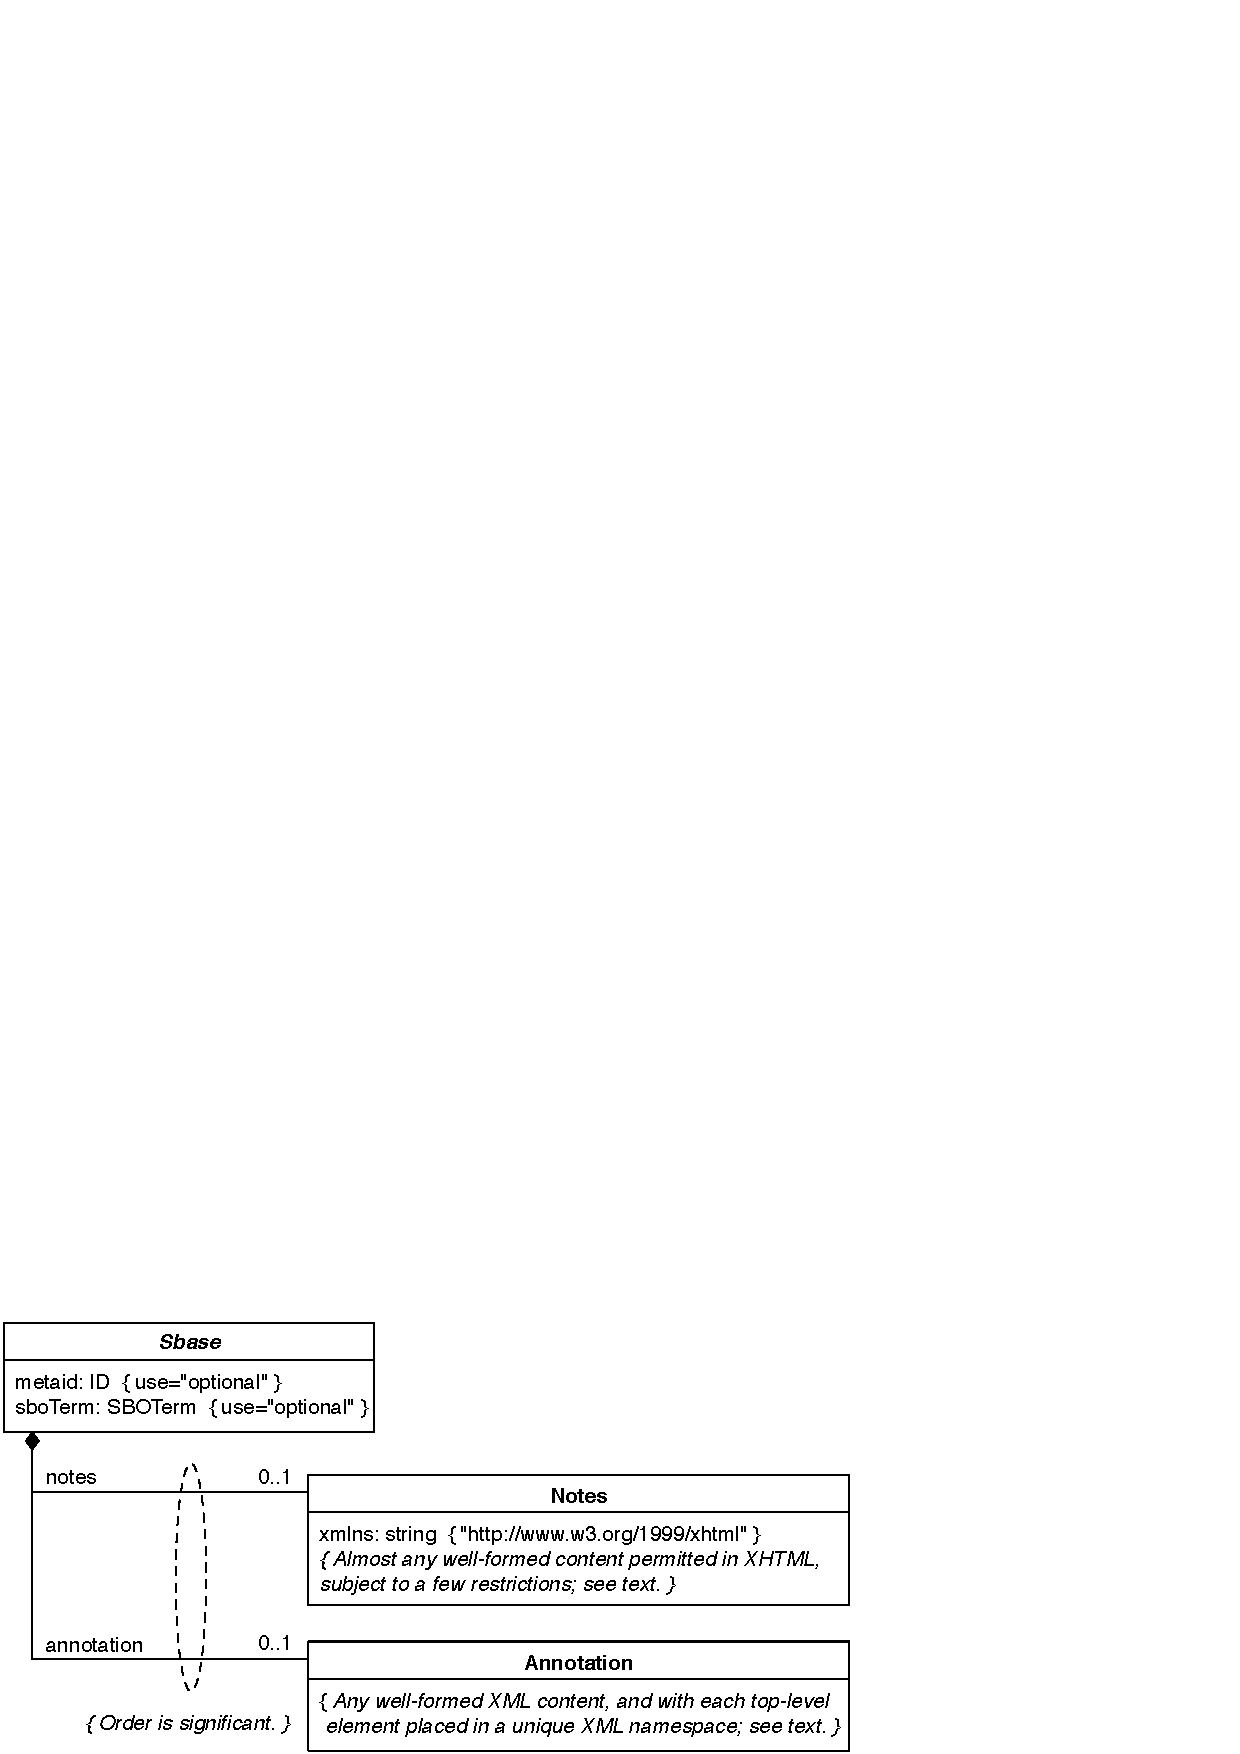
\includegraphics[scale=0.8]{figs/sbase-uml}
  \caption{The definition of \SBase.  Please refer to
    Section~\protect\ref{sec:notation} for a summary of the UML
    notation used here.}
  \label{fig:sbase}
\end{figure}

\SBase contains two attributes and two subelements, all of which
are optional: \token{metaid}, \token{sboTerm}, \Notes and
\Annotation.  These are discussed separately in the following
subsections.


\subsubsection{The \token{metaid} attribute}
\label{sec:metaid}

The \token{metaid} attribute is present for supporting metadata
annotations using RDF~\citep[Resource Description
Format;][]{lassila:1999}.  It has a data type of XML \token{ID}
(the XML identifier type; see Section~\ref{sec:id}), which means
each \token{metaid} value must be globally unique within an SBML
file.  The \token{metaid} value serves to identify a model
component for purposes such as referencing that component from
metadata placed within \token{annotation} elements (see
Section~\ref{sec:annotation-use}).  Such metadata can use RDF
\token{description} elements, in which an RDF attribute called
\val{rdf:about} points to the \token{metaid} identifier of an
object defined in the SBML model.  This topic is discussed in
greater detail in Section~\ref{sec:annotation-standard}.


\subsubsection{The \token{sboTerm} attribute}
\label{sec:sbase-sboterm}

The attribute called \token{sboTerm} is provided on \SBase to
support the use of the Systems Biology Ontology (SBO; see
Section~\ref{sec:sbo}).  When a value is given to this attribute,
it must conform to the data type \primtype{SBOTerm}
(Sections~\ref{sec:sboterm-type}).  SBO terms are a type of
optional annotation, and each different class of SBML object
derived from \SBase imposes its own requirements about the values
permitted for \token{sboTerm}.  Specific details on the permitted
values are provided with the definitions of SBML classes
throughout this specification document, and a broader discussion
is provided in Section~\ref{sec:sbo}.


\subsubsection{\class{Notes}}
\label{sec:notes}

The subcomponent \Notes in \SBase is a container for
XHTML~1.0~\citep{pemberton:2002} content.  It is intended to serve
as a place for storing optional information intended to be seen by
humans.  An example use of \Notes would be to contain formatted
user comments about the model element in which the \Notes object
is enclosed.  Every object derived directly or indirectly from
type \SBase can have a separate \Notes object instance, allowing
users considerable freedom when adding comments to their models.

% XHTML~1.0 is simply a formulation of HTML~4 in XML~1.0.  This
% means the full power of HTML formatting is available for use in
% \token{notes} content.  The intention behind requiring XHTML
% (rather than, for example, plain HTML or plain text) for
% \token{notes} content is to balance several conflicting goals: (1)
% choosing a format for notes that is compatible with the XML form of
% SBML (plain HTML would not be); (2) supporting an international
% formatting standard so that users have more control over the
% appearance of notes and can predict to some degree how their notes
% will be displayed in different tools and environments (which
% argues against using plain-text notes); and (3) achieving these
% goals using an approach that is hopefully easy enough for software
% developers to support using off-the-shelf programming libraries.
% It is worth noting in passing that the requirement for XHTML does
% not \emph{prevent} users from entering plain-text content with
% simple space/tab/newline formatting: it merely requires using the
% standard \token{<pre>}...\token{</pre>} element of (X)HTML.

% Modern libraries for displaying and editing (X)HTML content are
% commonly available in contemporary software programming
% environments, and software developers may wish to avail themselves
% of these facilities rather than implementing their own XHTML
% support systems.


\paragraph{XML namespace requirements for notes}

In XML, the \token{notes} elements must declare the use of
the XHTML XML namespace.  This can be done in multiple ways.  One
way is to place a namespace declaration for the appropriate
namespace URI (which is \uri{http://www.w3.org/1999/xhtml}) on the
top-level \Sbml object (see Section~\ref{sec:sbml}) and then
reference the namespace in the \token{notes} content using a
prefix.  The following example illustrates this approach:

\begin{example}
<sbml xmlns="http://www.sbml.org/sbml/level\sbmllevel/version\sbmlversionnum/core" level="\sbmllevel" version="\sbmlversionnum"
      xmlns:xhtml="http://www.w3.org/1999/xhtml">
  ...
  <notes>
    <xhtml:body>
      <xhtml:center><xhtml:h2>A Simple Mitotic Oscillator</xhtml:h2></xhtml:center>
      <xhtml:p>A minimal cascade model for the mitotic oscillator
      involving cyclin and cdc2 kinase</xhtml:p>
    </xhtml:body>
  </notes>
  ...
\end{example}

Another approach is to declare the XHTML namespace within the
\token{notes} content itself, as in the following example:

\begin{example}
...
<notes>
  <body xmlns="http://www.w3.org/1999/xhtml">
    <center><h2>A Simple Mitotic Oscillator</h2></center>
    <p>A minimal cascade model for the mitotic oscillator
    involving cyclin and cdc2 kinase</p>
  </body>
</notes>
...
\end{example}

The \token{xmlns="http://www.w3.org/1999/xhtml"} declaration on
\token{body} as shown above changes the default XML namespace
within it, such that all of its content is by default in the XHTML
namespace.  This is a particularly convenient approach because it
obviates the need to prefix every element with a namespace prefix
(\ie \val{xhtml:} in the earlier example).  Other
approaches are also possible.


\paragraph{The XHTML content of \class{notes}}

SBML does not require the content of a \Notes object to be any
particular XHTML element; the content can be almost any
well-formed XHTML content.  There is only one simple restriction,
and it comes from the requirements of XML: the \token{notes}
element must not contain an XML declaration nor a DOCTYPE
declaration.  That is, \token{notes} must \emph{not} contain

\begin{example}
<?xml version="1.0" encoding="UTF-8"?>  
\end{example}

nor the following (where the following is only one specific
example of a DOCTYPE declaration):

\begin{example}
<!DOCTYPE html PUBLIC "-//W3C//DTD XHTML 1.0 Strict//EN"
 "http://www.w3.org/TR/xhtml1/DTD/xhtml1-strict.dtd">
\end{example}


\subsubsection{\class{Annotation}}
\label{sec:annotation-use}
\label{sec:annotations}

Whereas \Notes is a container for content to be shown directly to
humans, \Annotation is a container for optional software-generated
content \emph{not} meant to be shown to humans.  Every object
derived from \SBase can have its own \Annotation object instance.
In XML, the \Annotation content type is \token{any}, allowing
essentially arbitrary well-formed XML data content.  SBML places
only a few restrictions on the organization of the content; these
are intended to help software tools read and write the data as
well as help reduce conflicts between annotations added by
different tools.


\paragraph{The use of XML namespaces in annotations}

% FIXME 2006-03-19:
% we should mention that RDF is an additional thing that can show
% up in annotations.  basically what's happening here is that we're
% saying any/all rdf content must be lumped together in one place

At the outset, software developers should keep in mind that
multiple software tools may attempt to read and write annotation
content.  To reduce the potential for collisions between
annotations written by different applications, SBML \thisLV
stipulates that tools must use XML namespaces~\citep{bray:1999} to
specify the intended vocabulary of every annotation.  The
application's developers must choose a URI (\emph{Universal
  Resource Identifier}; \citealt{harold:2001,w3c:2000}) reference
that uniquely identifies the vocabulary the application will use,
and a prefix string for the annotations.  Here is an example.
Suppose an application uses the URI \uri{http://www.mysim.org/ns}
and the prefix \token{mysim} when writing annotations related to 
molecules.  The content of an annotation might look like the
following:

\begin{example}
<annotation>
    <mysim:molecule xmlns:mysim="http://www.mysim.org/ns"
         mysim:weight="18.02" mysim:atomCount="3"/>
</annotation>
\end{example}

In this particularly simple example, the content consists of a single
XML element (\token{molecule}) with two attributes
(\token{weight}, \token{atomCount}), all of which are prefixed by
the string \token{mysim}.  (Presumably this particular content
would have meaning to the hypothetical application in question.)
The content in this particular example is small, but it should be
clear that there could easily have been an arbitrarily large
amount of data placed inside the \token{mysim:molecule} element.

The key point of the example above is that application-specific
annotation data are entirely contained inside a single
\emph{top-level element} within the SBML \token{annotation}
container.  SBML \thisLVnum places the following
restrictions on annotations:
\begin{itemize}

\item Within a given SBML \token{annotation} element, there can
  only be one top-level element using a given namespace.  An
  annotation element can contain multiple top-level elements but
  each must be in a different namespace.

% \item No top-level element in an \token{annotation} may use an
%   SBML XML namespace, either explicitly by referencing one of the
%   SBML XML namespace URIs or implicitly by failing to specify any
%   namespace on the annotation.  As of SBML \thisLV, the
%     defined SBML namespaces are the following URIs: \todo{MH}{need
%       to mention L3 packages too}
%   \begin{itemize}\setlength{\parskip}{-0.2ex}
%   \item \uri{http://www.sbml.org/sbml/level1}
%   \item \uri{http://www.sbml.org/sbml/level2}
%   \item \uri{http://www.sbml.org/sbml/level2/version2}
%   \item \uri{http://www.sbml.org/sbml/level2/version3}
%   \item \uri{http://www.sbml.org/sbml/level2/version4}
%   \item \uri{http://www.sbml.org/sbml/level3/version1/core}
%   \end{itemize}
  
\item The ordering of top-level elements within a given
  \token{annotation} element is \emph{not} significant.  An
  application should not expect that its annotation content
  appears first in the \token{annotation} element, nor in any
  other particular location.  Moreover, the ordering of
    top-level annotation elements may be changed by
  different applications as they read and write the same
    SBML file.

\end{itemize}

The use of XML namespaces in this manner is intended to improve
the ability of multiple applications to place annotations on SBML
model elements with reduced risks of interference or name
collisions.  Annotations stored by different simulation packages
can therefore coexist in the same model definition.  The rules
governing the content of \token{annotation} elements are designed
to enable applications to easily add, change, and remove their
annotations from SBML elements while simultaneously preserving
annotations inserted by other applications when mapping SBML from
input to output.

As a further simplification and to improve software
interoperability, applications are only required to preserve other
annotations (i.e., annotations they do not recognize) when those
annotations are self-contained entirely within \token{annotation},
complete with namespace declarations.  The following is an
example:

\begin{example}
<annotation>
    <topLevelElement xmlns="URI">
       \textrm{\emph{... content in the namespace identified by \textquotedblleft{}URI\textquotedblright}...}
    </topLevelElement>
</annotation>
\end{example}

Some more examples hopefully will make these points more clear.
The following example is invalid because it contains two top-level
elements using the same XML namespace.  Note that it does not
matter that these are two different top-level elements
(\token{<molecule>} and \token{<atom>}); what matters for
SBML is that these separate elements are both in the same
namespace rather than having been collected and placed inside one
overall container element for that namespace:

\begin{example}
<annotation>
    <mysim:molecule xmlns:mysim="http://www.mysim.org/ns"
        mysim:weigth="18.02" mysim:atomCount="3"/>
    <mysim:atom xmlns:mysim="http://www.mysim.org/ns"
        mysim:weight="18.02" mysim:atomCount="3"/>
</annotation>
\end{example}

On the other hand, the following example is valid:

\begin{example}
<annotation>
    <mysim:molecule xmlns:mysim="http://www.mysim.org/ns" mysim:weight="18.02" mysim:atoms="3"/>
    <struct:bonds xmlns:size="http://www.struct.org/ns" struct:number="2" struct:type="ionic" />
    <othersim:icon xmlns:othersim="http://www.othersim.com/">WS2002</othersim:icon>
</annotation>
\end{example}

For completeness, we note that annotations legally can be
empty (but such annotations have no meaning):

\begin{example}
<annotation />
\end{example}

It is worth keeping in mind that although XML namespace names must
be URIs, they are (like all XML namespace names) \emph{not
  required} to be directly usable in the sense of identifying an
actual, retrieval document or resource on the
Internet~\citep{bray:1999}.  URIs such as
\uri{http://www.mysim.org/} may appear as though they are (\eg)
Internet addresses, but there are not the same thing.  This style
of URI strings, using a domain name and other parts, is only a
simple and commonly-used way of creating a unique name string.

Finally, note that the namespaces being referred to here are XML
namespaces specifically in the context of the \token{annotation}
element on \SBase.  The namespace issue here is unrelated to the
namespaces discussed in Section~\ref{sec:identifiers} in the
context of component identifiers in SBML.


\paragraph{Content of annotations and implications for software tools}

\Annotation exists as a subobject of \SBase in
order that software developers may attach optional
application-specific data to the elements in an SBML model.
However, it is important that this facility not be misused.  In
particular, it is \emph{critical} that data essential to a model
definition or that can be encoded in existing SBML elements is
\emph{not} stored in annotations.  Parameter values,
functional dependencies between model elements, etc., should not
be recorded as annotations.  It is crucial to keep in mind the
fact that data placed in annotations can be freely ignored by
software applications.  If such data affect the interpretation of
a model, then software interoperability is greatly impeded.  
Recommendations regarding the use of any sort of annotation are
given in Section~\ref{sec:bp:annotations}.  


%-----------------------------------------------------------------------------
\subsection{The \token{id} and \token{name} attributes on SBML components}
\label{sec:idnameattribs}
%-----------------------------------------------------------------------------

As will become apparent below, most objects in SBML include two
common attributes: \token{id} and \token{name}.  These attributes are not
defined on \SBase (as explained in
Section~\ref{sec:why-not-on-sbase} below), but where they do
appear, the common rules of usage described below apply.


\subsubsection{The \token{id} attribute and identifier scoping}
\label{sec:identifiers}

The \token{id} attribute is mandatory on most (but not all)
objects in SBML.  It is used to identify a component within the
model.  Other SBML objects can refer to the component using this
identifier.  The data type of \token{id} is always either
\primtype{SId} (Section~\ref{sec:sid}) or \primtype{UnitSId}
(Section~\ref{sec:unitsid}), depending on the object in question.

A model can contain a large number of components representing
different parts.  This leads to a problem in deciding the scope of
an identifier: in what contexts does a given identifier \emph{X}
represent the same thing?  The approaches used in existing
simulation packages tend to fall into two categories which we may
call global and local.  The \emph{global} approach places all
identifiers into a single global space of identifiers, so that an
identifier \emph{X} represents the same thing wherever it appears
in a given model definition.  The \emph{local} approach places
symbols in separate identifier namespaces, depending on the
context, where the context may be, for example, individual
reaction rate expressions.  The latter approach means that a model
may use the same identifier \emph{X} in different rate expressions
and have each instance represent a different quantity.

The scoping rules in \sbmlthree are intended as a compromise to help
support both scenarios:
\begin{itemize}
  
\item The identifier (\ie the value of the attribute \token{id}) of
  every \FunctionDefinition, 
  \Compartment, \Species, \Parameter, \Reaction,
  \SpeciesReference, \ModifierSpeciesReference, \Event, and
  \Model, must be unique across the set of all such identifiers in
  the model.  This means, for example, that a reaction and a
  species definition cannot both have the same identifier.

\item The identifier of every \UnitDefinition must be unique
  across the set of all such identifiers in the model.  However,
  unit identifiers live in a separate space of identifiers from
  other identifiers in the model, by virtue of the fact that the
  data type of unit identifiers is \primtype{UnitSId}
  (Section~\ref{sec:unitsid}) and not \primtype{SId}.
  
\item Each \Reaction instance (see Section~\ref{sec:reactions})
  establishes a separate private local space for local parameters
  represented by objects of class \LocalParameter.  Within the
  definition of that reaction, local parameter identifiers
  override (shadow) identical identifiers (whether those
  identifiers refer to parameters, species or compartments)
  outside of that reaction.  Of course, the corollary of this is
  that local parameters inside a \Reaction object instance are not
  visible to other objects outside of that reaction.

\end{itemize}


\subsubsection{The \token{name} attribute}
\label{sec:name}

In contrast to the \token{id} attribute, the \token{name} attribute is
optional and is not intended to be used for cross-referencing
purposes within a model.  Its purpose instead is to provide a
human-readable label for the component.  The data type of 
\token{name} is the type \primtype{string} defined in XML
Schema~\citep{biron:2000,thompson:2000} and discussed further in
Section~\ref{sec:primitive-types}.  SBML imposes no restrictions
as to the content of \token{name} attributes beyond those restrictions
defined by the \primtype{string} type in XML Schema.
In addition, there are no restrictions on the uniqueness
of \token{name} values in a model (unlike the restrictions on
\token{id} values discussed in Section~\ref{sec:identifiers}).


\subsubsection{Why \token{id} and \token{name} are not defined on \class{SBase}}
\label{sec:why-not-on-sbase}

Although many SBML components feature \token{id} and \token{name},
these attributes are purposefully not defined on \SBase.  There
are several reasons for this.
\begin{itemize}
  
\item The presence of an SBML identifier attribute (\token{id})
  necessarily requires specifying scoping rules for the
  corresponding identifiers.  However, the \SBase abstract type is
  used as the basis for defining components whose scoping rules
  are in some cases different from each other.  (See
  Section~\ref{sec:identifiers} for more details).  If \SBase were
  to have an \token{id} attribute, then the specification of \SBase
  would need a default scoping rule and this would then have to be
  overloaded on derived classes that needed different scoping.
  This would make the SBML specification even more complex.
  
\item Identifiers are optional on some SBML components and required
  on most others.  If \token{id} were defined as optional on
  \SBase, most component classes would separately have to redefine
  \token{id} as being mandatory---hardly an improvement over the
  current arrangement.  Conversely, if \token{id} were defined as
  mandatory on \SBase, it would prevent it from being optional on
  components where it \emph{is} currently optional.
  
\item The \SBase abstract type is used as the base type for
  certain objects such as \Sbml, \AssignmentRule,
  etc., which do not have identifiers because these components do
  not need to be referenced by other components.  If \SBase had a
  mandatory \token{id} attribute, \emph{all} objects of
  these other types in a model would then need to be assigned
  unique identifiers.  Similarly, because \SBase is the
    base type of the \token{listOf\rule{0.5in}{0.5pt}} lists,
  putting \token{id} on \SBase would require all of these lists in
  a model to be given identifiers.  This would be a needless
  burden on software developers, tools, and SBML users, requiring
  them to generate and store additional identifiers for objects
  that never need them.
  
\item \SBase does not have a \token{name} simply because such an
  attribute is always paired with an \token{id}.  Without
  \token{id} on \SBase, it does not make sense to have
  \token{name}.

\end{itemize}


%-----------------------------------------------------------------------------
\subsection{Mathematical formulas in SBML Level 3}
\label{sec:formulas}
%-----------------------------------------------------------------------------

Mathematical expressions in SBML Level~3 are represented using
\mathmltwo~\citep{w3c:2000b}.  MathML is an international standard
for encoding mathematical expressions using XML.  There are two
principal facets of MathML, one for encoding content (\ie the
semantic interpretation of a mathematical expression), and another
for encoding presentation or display characteristics.  SBML only
makes direct use of a subset of the content portion of MathML.
However, it is not possible to produce a completely smooth and
conflict-free interface between MathML and other standards used by
SBML (in particular, \xmlschema).  Two specific issues and their
resolutions are discussed in Sections~\ref{sec:cn-token}.

The XML namespace URI for all MathML elements is
\uri{http://www.w3.org/1998/Math/MathML}.  Everywhere MathML
content is allowed in SBML, the MathML elements must be properly
placed within the \mathmltwo namespace.  In XML, this can be
accomplished in a number of ways, and the examples throughout this
specification illustrate the use of this namespace and MathML in
SBML.  Please refer to the W3C document by \citet{bray:1999} for
more technical information about using XML namespaces.


\subsubsection{Subset of MathML used in SBML Level 3}
\label{sec:mathmlsubset}

The subset of MathML elements used in SBML is listed below:
\begin{itemize}\setlength{\parskip}{-0.1ex}

\item \emph{token}: \token{cn}, \token{ci}, \token{csymbol},
  \token{sep}
  
\item \emph{general}: \token{apply}, \token{piecewise},
  \token{piece}, \token{otherwise}, \token{lambda} (however, as
  discussed elsewhere, \token{lambda} is restricted to use in
  \FunctionDefinition)

\item \emph{relational operators}: \token{eq}, \token{neq},
  \token{gt}, \token{lt}, \token{geq}, \token{leq}

\item \emph{arithmetic operators}: \token{plus}, \token{minus},
  \token{times}, \token{divide}, \token{power}, \token{root},
  \token{abs}, \token{exp}, \token{ln}, \token{log},
  \token{floor}, \token{ceiling}, \token{factorial}

\item \emph{logical operators}: \token{and}, \token{or},
  \token{xor}, \token{not}

\item \emph{qualifiers}: \token{degree}, \token{bvar},
  \token{logbase}

\item \emph{trigonometric operators}: \token{sin}, \token{cos},
  \token{tan}, \token{sec}, \token{csc}, \token{cot},
  \token{sinh}, \token{cosh}, \token{tanh}, \token{sech},
  \token{csch}, \token{coth}, \token{arcsin}, \token{arccos},
  \token{arctan}, \token{arcsec}, \token{arccsc}, \token{arccot},
  \token{arcsinh}, \token{arccosh}, \token{arctanh},
  \token{arcsech}, \token{arccsch}, \token{arccoth}

\item \emph{constants}: \token{true}, \token{false},
  \token{notanumber}, \token{pi}, \token{infinity},
  \token{exponentiale}

\item \emph{MathML annotations}: \token{semantics},
  \token{annotation}, \token{annotation-xml}

\end{itemize}

The inclusion of logical operators, relational operators,
\token{piecewise}, \token{piece}, and \token{otherwise} elements
facilitates the encoding of discontinuous expressions.

As defined by \mathmltwo, the semantic interpretation of the
mathematical functions listed above follows the definitions of the
functions laid out by \cite{abramowitz:1997} and
\cite{zwillinger:1988}.  Readers are directed to these sources and
the MathML specification for information about such things as
which principal values of the inverse trigonometric functions to
use.

Software authors should take particular note of the MathML
semantics of the N-ary operators \token{plus}, \token{times},
\token{and}, \token{or} and \token{xor}, when they are used with
different numbers of arguments.  The MathML
specification~\citep{w3c:2000b} appendix C.2.3 describes the
semantics for these operators with zero, one, and more arguments.

The following are the only attributes permitted on MathML elements
in SBML (in addition to the \token{xmlns} attribute on
\token{math} elements):
\begin{itemize}\setlength{\parskip}{-0.2ex}

\item \token{style}, \token{class} and \token{id} on any element;

\item \token{encoding} on \token{csymbol},
    \token{annotation} and \token{annotation-xml} elements;

\item \token{definitionURL} on \token{ci}, \token{csymbol}
    and \token{semantics} elements; and

\item \token{type} and \token{sbml:units}
  (see Section~\ref{sec:cn-token}) on \token{cn} elements.

\end{itemize}\vspace*{-0.75ex}
Missing values for the MathML attributes are to be treated in the
same way as defined by MathML~2.0.  These restrictions on
attributes are designed to confine the MathML elements to their
default semantics and to avoid conflicts in the interpretation of
the type of token elements.


\subsubsection{Numbers and \token{cn} elements}
\label{sec:cn-token}
\label{sec:mathml-value-space}

In MathML, literal numbers are written as the content portion of a
particular element called \token{cn}.  This element takes an
optional attribute, \token{type}, used to indicate the \emph{type}
of the number (such as whether it is meant to be an integer or a
floating-point quantity).  Here is an example of its use:

\begin{example}
<math xmlns="http://www.w3.org/1998/Math/MathML">
    <apply>
        <times/> <cn type="integer"> 42 </cn> <cn type="real"> 3.3 </cn>
    </apply>
</math>
\end{example}

The content of a \token{cn} element must be a number.  The number
can be preceded and succeeded by whitespace (see
Section~\ref{sec:mathml-whitespace}).  The following are the only
permissible values for the \token{type} attribute on MathML
\token{cn} elements: \val{e-notation}, \val{real}, \val{integer},
and \val{rational}.  The value of the \token{type} attribute
defaults to \val{real} if it is not specified on a given
\token{cn} element.


\paragraph{Value space restrictions on \token{cn} content}

SBML imposes certain restrictions on the value space of numbers
allowed in MathML expressions.  According to the \mathmltwo
specification, the values of the content of \token{cn} elements do
not necessarily have to conform to any specific floating point or
integer representations designed for CPU implementation.  For
example, in strict MathML, the value of a \token{cn} element could
exceed the maximum value that can be stored in a IEEE 64 bit
floating point number (IEEE 754).  This is different from the XML
Schema type \primtype{double} that is used in the definition of
floating point attributes of objects in SBML; the XML Schema
\primtype{double} \emph{is} restricted to IEEE double-precision
64-bit floating point type IEEE 754-1985.  To avoid an
inconsistency that would result between numbers elsewhere in SBML
and numbers in MathML expressions, SBML \thisLV imposes the
following restriction on MathML content appearing in SBML:
\begin{itemize}
  
\item Integer values (\ie the values of \token{cn} elements
  having \token{type}=\val{integer} and both values in \token{cn} elements
  having \token{type}=\val{rational}) must conform to the
  \primtype{int} type used elsewhere in SBML
  (Section~\ref{sec:integer})
  
\item Floating-point values (\ie the content of \token{cn}
  elements having \token{type}=\val{real} or
  \token{type}=\val{e-notation}) must conform to the
  \primtype{double} type used elsewhere in SBML
  (Section~\ref{sec:double})
\end{itemize}


\paragraph{Syntactic differences in the representation of numbers
  in scientific notation}

It is important to note that MathML uses a style of scientific
notation that differs from what is defined in XML Schema, and
consequently what is used in SBML attribute values.  The
\mathmltwo type \val{e-notation}
(as well as the type \val{rational})
requires the mantissa and
exponent to be separated by one \texttt{<sep/>} element.  The
mantissa must be a real number and the exponent part must be a
signed integer.  This leads to expressions such as

\begin{example}
<cn type="e-notation"> 2 <sep/> -5 </cn>
\end{example}

for the number $2 \cdot 10^{-5}$.  It is especially
important to note that the following expression,

\begin{example}
<cn type="e-notation"> 2e-5 </cn>
\end{example}

is \emph{not valid} in \mathmltwo and therefore cannot be used in
MathML content in SBML.  However, elsewhere in SBML, when an
attribute value is declared to have the data type
\primtype{double} (a type taken from XML Schema), the compact
notation \val{2e-5} is in fact allowed.  In other words, within
MathML expressions contained in SBML (and \emph{only} within such
MathML expressions), numbers in scientific notation must take the
form \token{<cn type="e-notation"> 2 <sep/> -5 </cn>}, and
everywhere else they must take the form \val{2e-5}.

This is a regrettable difference between two standards that SBML
replies upon, but it is not feasible to redefine these types
within SBML because the result would be incompatible with parser
libraries written to conform with the MathML and XML Schema
standards.  It is also not possible to use XML Schema to define a
data type for SBML attribute values permitting the use of the
\token{<sep/>} notation, because XML attribute values cannot
contain XML elements---that is, \token{<sep/>} cannot appear in an
XML attribute value.


\paragraph{Units associated with numbers in MathML \token{cn} expressions}
\label{sec:units-of-mathml}

What units should be attributed to numbers appearing inside MathML
\token{cn} elements?  One answer is to assume that the units
should be ``whatever units appropriate in the context where the
number appears''.  This implies that units can always be assigned
unambiguously to any number by inspecting the expression in which
it appears, and this turns out to be false.  Another answer is
that numbers should be considered ``dimensionless''.  Many people
argue that this is the correct interpretation, but even if it is,
there is an overriding practical reason why it cannot be adopted
for SBML's domain of application: when numbers appear in
expressions in SBML, they are \emph{rarely intended} by the
modeler to have the unit \val{dimensionless} even if the unit is
not declared---instead, the numbers are \emph{supposed} to have
specific units, but the units are usually undeclared.  (Being
``dimensionless'' is not the same as having \emph{undeclared}
units!)  If SBML defined numbers as being \emph{by default}
dimensionless, it would result in many models being technically
incorrect without the modeler being aware of it unless their
software tools performed dimensional analysis.  Many software
tools do not perform unit analysis, and so potential errors due to
inconsistent units in a model would not be detected until other
researchers and database curators attempted to use the model in
software packages that \emph{did} check units.  We believe the
negative impact on interoperability would be too high.

SBML borrows an idea from CellML~\citep{hedley:2001b}, another
model definition language with similar goals as SBML, and allows
an additional attribute to appear on MathML \token{cn} elements;
the value of this attribute can be used to indicate the units
associated with the number in the content of the \token{cn}
element.  The attribute is named \token{units} but, because it
appears inside MathML element (which is in the XML namespace for
MathML and not the namespace for SBML), it must always be prefixed
with an XML namespace prefix for the SBML \thisLV namespace.  The
value of the attribute must have the data type
\primtype{UnitSIdRef} (Section~\ref{sec:unitsidref}) and can be
the identifier of a \UnitDefinition object in the model or a base
unit listed in Table~\vref{tab:unitkind}.  The following example
illustrates how this attribute can be used to define a number with
value \val{10} and unit of measurement \val{second}:
\vspace*{-0.5ex}
\begin{example}
<math xmlns="http://www.w3.org/1998/Math/MathML"
      xmlns:sbml="http://www.sbml.org/sbml/level3/version1/core">
    <cn type="integer" sbml:units="second"> 10 </cn>
</math>
\end{example} 
\vspace*{-0.5ex}
In this example, we chose to use the string \val{sbml} as the XML
namespace prefix for the SBML \thisLV namespace, which leads to
the use of \token{sbml:units} as the attribute on the \token{cn}
element.  We could have used another prefix string besides
\val{sbml}, and the definition of the prefix could also have
appeared on a higher-level element in the model.
Section~\ref{sec:sbml} provides more information about the XML
namespace for SBML \thisLV.

An alternative approach to specifying units is to avoid using
\token{cn} elements altogether, and always use \token{ci} elements
to reference \Parameter objects having both value and units
defined.  In the example above, we could have avoided putting the
literal number \val{10} inside the mathematical expression, and
instead, defined a parameter in the model, given it the value
\val{10} and unit \val{second}, and finally, referred to that
parameter in the \token{math} content above.  The approach of
using named parameters provides additional power and advantages
over simply using \token{sbml:units} attributes on \token{cn}
elements; for example, \Parameter allows the association of terms
from the Systems Biology Ontology (SBO; Section~\ref{sec:sbo}) as
well as MIRIAM annotations (Section~\ref{sec:annotations}).

In summary, a literal number within MathML content without an SBML
\token{units} attribute has no declared units.  Either of the two
approaches described above (\ie avoiding \token{cn} in favor of
\token{ci} elements and \Parameter objects, or using \token{cn}
with a \token{sbml:units} attribute) leads to mathematical
formulas whose units can be fully determined, enabling software
tools to perform dimensional analysis and, potentially, detect and
report problems with the model.  Conversely, in the absence of an
SBML \token{units} attribute on a MathML \token{cn} element, no
units are associated with the number within the \token{cn}
element; in other words, \emph{the units are undeclared}.  If the
example above lacked the attribute \token{sbml:units}, the value
\val{10} would have no declared units.

Finally, although SBML provides ways of associating units with
numbers and entities, SBML does not stipulate that implicit unit
conversions be performed.
Section~\ref{sec:no-implicit-conversions} explores this topic in
more detail.


\subsubsection{Use of \token{ci} elements in MathML expressions in SBML}
\label{sec:ci-token}

The content of a \token{ci} element must be an SBML identifier
that is declared elsewhere in the model.  The identifier can be
preceded and succeeded by whitespace within the \token{ci}.  The
set of possible identifiers that can appear in a \token{ci}
element depends on the containing element in which the \token{ci}
is used:
\begin{itemize}
  
\item If a \token{ci} element appears in the \token{math} body of
  a \FunctionDefinition object
  (Section~\ref{sec:functiondefinition}), the referenced
  identifier must be either (i) one of the declared arguments to
  that function, or (ii) the identifier of another
  \FunctionDefinition object in the model.
  
\item Otherwise, the referenced identifier must be that of a
  \Compartment, \FunctionDefinition, \Parameter, \Reaction,
  \Species or \SpeciesReference object defined in the model.  The
  following are the only possible interpretations of using such an
  identifier in SBML:
  \begin{itemize}

  \item \emph{Compartment identifier}: When a \Compartment
    identifier occurs in a \token{ci} element, it represents the
    size of the compartment.  The units of measurement associated
    with the size of the compartment are those given by the
    \Compartment instance's \token{units} attribute value; see
    Section~\ref{sec:compartment-units}.
    
  \item \emph{Function identifier}: When a \FunctionDefinition
    identifier occurs in a \token{ci} element, it represents a
    call to that function.  Function references in MathML occur in
    the context of using MathML's \token{apply} and often involve
    supplying arguments to the function; see
    Section~\ref{sec:functiondefinition}.  The units associated
    with the value returned by the function call are the overall
    units of the mathematical expression contained in the function
    definition.
    
  \item \emph{Parameter identifier}: When a \Parameter identifier
    occurs in a \token{ci} element, it represents the numerical
    value assigned to that parameter.  The units associated with
    the parameter's value are those given by the
      \Parameter instance's \token{units} attribute; see
    Section~\ref{sec:parameter-units}.

  \item \emph{Reaction identifier}: When a \Reaction identifier
    occurs in a \token{ci} element, it represents the rate of that
    reaction as defined by the \token{math} expression in the
    \KineticLaw object within the \Reaction.  The units associated
    with that rate are \emph{extent units}/\emph{time units},
    where the \emph{extent units} are given by the \Model
    attribute \token{extentUnits}
    (Section~\ref{sec:model-extentUnits}) and \emph{time units}
    are given by the \Model attribute token{timeUnits}
    (Section~\ref{sec:model-timeUnits}).  If a \Reaction instance
    has no \KineticLaw, using its reaction identifier this way is
    an error.
    
  \item \emph{Species identifier}: When a \Species identifier
    occurs in a \token{ci} element, it represents the quantity of
    that species in units of either \quantity{amount of substance}
    or \quantity{concentration}, depending on the
    species' definition; see Section~\ref{sec:species-units}.

  \item \emph{Species reference identifier}: When a
    \SpeciesReference identifier occurs in a \token{ci} element,
    it represents the stoichiometry of the reactant or product in
    the reaction where the \SpeciesReference object is defined.
    More precisely, the value of the \SpeciesReference
    identifier is equal to the value of the \token{stoichiometry}
    attribute of that \SpeciesReference object instance; see
    Section~\ref{sec:reactions}.  The unit associated with the
    value is always \token{dimensionless}.
    
  \end{itemize}

\end{itemize}

The content of \token{ci} elements in MathML formulas outside of a
\KineticLaw or \FunctionDefinition must always refer to objects
declared in the top level global namespace; \ie SBML uses ``early
binding'' semantics.  Inside of \KineticLaw, \token{ci} elements
can additionally refer to identifiers of \LocalParameter objects
defined within that \KineticLaw instance; see
Section~\ref{subsec:kinetic-law} for more information.


\subsubsection{Interpretation of boolean values}
\label{sec:handling-booleans}

As noted already in Section~\ref{sec:boolean}, there is another
unfortunate difference between the \xmlschemaone and \mathmltwo
standards that impacts mathematical expressions in SBML: in
\xmlschema, the value space of type \primtype{boolean} includes
\val{true}, \val{false}, \val{1}, and \val{0}, whereas in
\mathml, only \val{true} and \val{false} count as boolean
values.

The impact of this difference thankfully is minimal because the
\xmlschema definition is only used for attribute values on SBML
objects, and those values turn out never to be accessible from
\mathml content in SBML---values of boolean attributes on SBML objects
can never enter into \mathml expressions.  Nevertheless, software
authors and users should be aware of the difference and in
particular that \val{0} and \val{1} are interpreted as numerical
quantities in mathematical expressions.  There is no automatic
conversion of \val{0} or \val{1} to boolean values in contexts
where booleans are expected.  This allows stricter type checking
and unit verification during the validation of mathematical
expressions.


\subsubsection{Handling of whitespace}
\label{sec:mathml-whitespace}

\mathmltwo defines ``whitespace'' in the same way as XML does, \ie
the space character (Unicode hexadecimal code 0020), horizontal
tab (code 0009), newline or line feed (code 000A), and carriage
return (code 000D).  In MathML, the content of elements such as
\token{cn} and \token{ci} can be surrounded by whitespace
characters.  Prior to using the content, this whitespace is
``trimmed'' from both ends: all whitespace at the beginning and
end of the content is removed~\citep{ausbrooks:2003}.  For
example, in \texttt{<cn> 42 </cn>}, the amount of white space on
either side of the ``\texttt{42}'' inside the \texttt{<cn>}
\ldots\ \texttt{</cn>} container does not matter.  Prior to
interpreting the content, the whitespace is removed altogether.


\subsubsection{Use of \token{csymbol} elements in MathML expressions in SBML}
\label{sec:csymbol-token}
\label{sec:csymbol}

SBML \thisL uses the MathML \token{csymbol} element to denote
certain built-in mathematical entities without introducing
reserved names into the component identifier namespace.  The
\token{encoding} attribute of \token{csymbol} must be set to
\val{text}.  The \token{definitionURL} should be set to one of the
following URIs defined by SBML:
\begin{itemize}

\item \uri{http://www.sbml.org/sbml/symbols/time}.  This
  represents the current simulation time.  See
  Section~\ref{sec:meaning-of-time} for more information.  The
  unit of measurement associated with time is determined by the
  value of the \token{timeUnits} attribute on \Model.

\item \uri{http://www.sbml.org/sbml/symbols/delay}.  This
  represents a delay function.  The delay function has the form
  $delay(x, d)$, taking two MathML expressions as arguments.  The
  function's value is the value of argument $x$, but taken at a
  time $d$ before the current time.  There are no restrictions on
  the form of $x$.  Since the parameter $d$ represents a time
  value, the units of $d$ are expected to match the time units of
  the model; those are in turn specified by the value of the
  attribute \token{timeUnits} on \Model.  The value of the $d$
  parameter, when evaluated, must be numerical (\ie a number in
  MathML real, integer, or ``e-notation'' format) and be greater
  than or equal to 0.  The units of the return value of the delay
  functions are those of the parameter $x$.  See
  Section~\ref{sec:meaning-of-time} below for additional
  considerations surrounding the use of this \token{csymbol}.

\item \uri{http://www.sbml.org/sbml/symbols/avogadro}.  This
  represents the numerical value of Avogadro's constant.  The
  value of Avogadro's constant is determined experimentally; for
  the purposes of SBML \thisLVnum, the numerical value is taken to
  be the one recommended by the 2006 edition of
  CODATA~\citep{codata_2008}, but the unit is
  \token{dimensionless}.  In other words, the value of this
  \token{csymbol} is equivalent to the following:
  \begin{linenomath}
    \begin{equation*}
      (6.02214179 \cdot 10^{23}) \cdot \texttt{dimensionless}
    \end{equation*}
  \end{linenomath}
  If the value of Avogadro's constant is revised by international
  standards-setting organizations in the future, a future Version
  of the SBML \thisL specification may stipulate a new value to be
  used for this \token{csymbol} constant.  However, all software
  reading models expressed in \emph{this} Version of SBML Level~3
  should \emph{always} use the value of Avogadro's constant given
  above.  (In other words, changes will apply only beginning with
  a possible new Version of SBML Level~3 and not this existing
  version.)

\end{itemize}

The following examples demonstrate these concepts.  The XML fragment below
encodes the formula $x + t$, where $t$ stands for time.

\begin{example}
<math xmlns="http://www.w3.org/1998/Math/MathML">
    <apply>
        <plus/>
        <ci> x </ci>
        <csymbol encoding="text" definitionURL="http://www.sbml.org/sbml/symbols/time">
            t
        </csymbol>
    </apply>
</math>
\end{example}

In the fragment above, the use of the token \token{t} is mostly a
convenience for human readers---the string inside the
\token{csymbol} could have been almost anything, because it is
essentially ignored by MathML parsers and SBML.  Some MathML and
SBML processors will take note of the token and use it when
presenting the mathematical formula to users, but the token used
has no impact on the interpretation of the model and it does
\emph{not} enter into the SBML component identifier namespace.  In
other words, the SBML model cannot refer to \token{t} in the
example above.  The content of the \token{csymbol} element is for
rendering purposes only and can be ignored by the parser.

As a further example, the following XML fragment encodes the equation
$k + delay(x, 0.1)$ or, alternatively, $k_t + x_{t - 0.1}$:

\begin{example}

<math xmlns="http://www.w3.org/1998/Math/MathML"
      xmlns:sbml="http://www.sbml.org/sbml/level3/version1/core">
    <apply>
        <plus/>
        <ci> k </ci>
        <apply>
            <csymbol encoding="text" definitionURL="http://www.sbml.org/sbml/symbols/delay">
                delay
            </csymbol>
            <ci> x </ci>
            <cn sbml:units="second"> 0.1 </cn>
        </apply>
    </apply>
</math>
\end{example}

Finally, the use of Avogadro's number is illustrated in the
following XML fragment:

\begin{example}
<math xmlns="http://www.w3.org/1998/Math/MathML">
    <apply>
        <times/>
        <apply>
            <csymbol encoding="text" definitionURL="http://www.sbml.org/sbml/symbols/avogadro">
                Avogadro's number
            </csymbol>
            <ci> x </ci>
        </apply>
    </apply>
</math>
\end{example}


\subsubsection{Simulation time}
\label{sec:meaning-of-time}

The principal use of SBML is to represent quantitative dynamical
models whose behaviors manifest themselves over time.  In defining
an SBML model using constructs such as reactions, time is most
often implicit and does not need to be referred to in the
mathematical expressions themselves.  However, sometimes an
explicit time dependency needs to be stated, and for this purpose,
the \emph{time} \token{csymbol} (described above in
Section~\ref{sec:csymbol-token}) may be used.  This \emph{time}
symbol refers to ``instantaneous current time'' in a simulation,
frequently given the literal name $t$ in one's equations.

An assumption in SBML is that ``start time'' or ``initial time''
in a simulation is zero, that is, if $t_0$ is the initial time in
the system, $t_0 = 0$.  This corresponds to the most common
scenario.  Initial conditions in SBML take effect at time $t = 0$.
There is no mechanism in SBML for setting the initial time to a
value other than 0.  To refer to a different time in a model, one
approach is to define a \Parameter for a new time variable and use
an \AssignmentRule in which the assignment expression subtracts a
value from the \token{csymbol} \emph{time}.  For example, if the
desired offset is 2 time units, the MathML expression would be

\begin{example}
<math xmlns="http://www.w3.org/1998/Math/MathML"
      xmlns:sbml="http://www.sbml.org/sbml/level3/version1/core">
    <apply>
        <minus/>
        <csymbol encoding="text" definitionURL="http://www.sbml.org/sbml/symbols/time"/> 
        <cn sbml:units="second"> 2 </cn>
    </apply>
</math>
\end{example}

SBML's assignment rules (Section~\ref{sec:assignmentrule}) can be
used to express mathematical statements that hold true at all
moments, so using an assignment rule with the expression above
will result in the value being equal to $t - 2$ at every point in
time.  A parameter assigned this value could then be used
elsewhere in the model.


\subsubsection{Initial conditions and special considerations}
\label{sec:before-t0}

The identifiers of \Species, \SpeciesReference, \Compartment, \Parameter, and
\Reaction object instances in a given SBML model refer to the main
variables in a model.  Depending on certain attributes of these
objects (\eg the attribute \token{constant} on species, species references, compartments
and parameters---this and other conditions are explained in the
relevant sections elsewhere in this document), some of the
variables may have constant values throughout a simulation, and
others' values may change.  These changes in values over time are
determined by the system of equations constructed from the model's
reactions, initial assignments, rules, and events.

As described in Section~\ref{sec:meaning-of-time}, an SBML model's
simulation is assumed to begin at $t = 0$.  The availability of
the \emph{delay} \token{csymbol} (Section~\ref{sec:csymbol-token})
introduces the possibility that at $t \geq 0$, mathematical
expressions in a model may draw on values of model components from
time \emph{prior} to $t = 0$.  A simulator may therefore need to
compute the values of variables at time points $t_i \leq 0$ to
allow the calculation of values required for the evaluation of
delay expressions in the model for $t \geq 0$.  If there are no
delays in the model, then $t_i = 0$.

The following is how the definitions of the model should be
applied:

%\todo{anyone}{revise to include speces ref id's}

\begin{enumerate}

\item At time $t_i$:
  \begin{itemize}
    
  \item Every \Species, \SpeciesReference, \Compartment, and \Parameter whose
    definition includes an initial value is assigned that value.
    If an element has \token{constant}=\val{false}, its
    value may be changed by other constructs or reactions in a
    model according to the steps below; if
    \token{constant}=\val{true}, only an \InitialAssignment can
    override the value.
    
  \item All \InitialAssignment definitions take effect at $t_i$
    and continue to have effect up to and including $t = 0$,
    overriding any initial values on \Species, \SpeciesReference,
    \Compartment, and \Parameter.  Since \InitialAssignment{}s
    contain mathematical formulas, different values may be
    computed at each time step $t$ in $t_i \leq t \leq 0$.

%    The value of every \Species, \Compartment, and \Parameter    
%    object whose identifier is \emph{not} the subject of an
%    \InitialAssignment is assigned by the definition of that
%    object in the model; conversely, the value of every \Species,
%    \Compartment, and \Parameter object whose identifier \emph{is}
%    the subject of an \InitialAssignment is computed and assigned
%    by that \InitialAssignment.  
%    All assignments of both kinds are
%    performed once and thereafter are in effect for $t \geq t_i$.

  \end{itemize}
  
\item For time $t \geq t_i$:
  \begin{itemize}
    
  \item \AssignmentRule and \AlgebraicRule definitions are in
    effect from this point in time forward and may influence the
    values of \Species quantity, \SpeciesReference stoichiometry,
    \Compartment size, and \Parameter
    values.  (Note there cannot be both an \AssignmentRule and an
    \InitialAssignment for the same identifier; see
    Section~\ref{sec:rules}.)

  \end{itemize}
  
\item At time $t = 0$:
  \begin{itemize}  
    
  \item The system of equations constructed by combining
    \AssignmentRule equations, \AlgebraicRule equations, \RateRule
    equations, and the equations constructed from the \Reaction
    definitions in the model, are used to obtain consistent
    initial conditions for numerical solver algorithms.  (Note
    that there cannot be both an \AssignmentRule and a \RateRule
    for the same identifier, or both an \AssignmentRule and an
    \InitialAssignment for the same identifier; see
    Section~\ref{sec:assignmentrule}.)
    
  \item \Constraint definitions begin to take effect (and a
    constraint violation may result; see
    Section~\ref{sec:constraints}).

  \end{itemize}
  
\item For time $t > 0$:
  \begin{itemize}
    
  \item \RateRule definitions can begin to take effect.
    
  \item \Event definitions can begin to take effect.  (Note that
    an \Event cannot be defined to change the value of a variable
    that is also the subject of an \AssignmentRule; see
    Section~\ref{sec:events}.)

  \item System simulation proceeds.

  \end{itemize}

\end{enumerate}  

To reiterate: in modeling situations that do not involve the use
of the \emph{delay} \token{csymbol}, then $t_i$ becomes $t_i = 0$,
but this does not alter the steps numbers 1--4 above.


\subsubsection{MathML expression data types}
\label{sec:mathmltype}

MathML operators in SBML each return results in one of two
possible types: boolean and numerical.  By
\emph{numerical} type, we mean either (1) a number in
  MathML real, integer, rational, or ``e-notation'' format;
or (2) the \token{csymbol} for delay or the
  \token{csymbol} for time described in
  Section~\ref{sec:csymbol-token}.  The following guidelines
summarize the different possible cases.

The relational operators (\token{eq}, \token{neq}, \token{gt},
\token{lt}, \token{geq}, \token{leq}), the logical operators
(\token{and}, \token{or}, \token{xor}, \token{not}), and the
boolean constants (\token{false}, \token{true}) always return
boolean values.  As noted in
  Section~\ref{sec:handling-booleans}, the numbers \token{0} and
  \token{1} do not count as boolean values in \mathml
  contexts in SBML.

The type of an operator referring to a \FunctionDefinition is
determined by the type of the top-level operator of the expression
in the \token{math} element of the \FunctionDefinition
instance, and can be boolean or numerical.

All other operators, values and symbols return numerical
results.

The roots of the expression trees used in the following contexts
must yield boolean values:

\begin{itemize}\setlength{\parskip}{-0.2ex}

\item the arguments of the MathML logical operators (\token{and},
\token{or}, \token{xor}, \token{not});

\item the second argument of a MathML \token{piece} operator;

\item the \token{trigger} element of an SBML \Event; and

\item the \token{math} element of an SBML \Constraint.

\end{itemize}

The roots of the expression trees used in the following contexts can
optionally yield boolean values:

\begin{itemize}\setlength{\parskip}{-0.2ex}

\item the arguments to the \token{eq} and \token{neq} operators;

\item the first arguments of MathML \token{piece} and \token{otherwise}
operators; and

\item the top level expression of a function definition.

\end{itemize}

The roots of expression trees in other contexts must yield
numerical values.

The type of expressions should be used consistently.  The set of
expressions that make up the first arguments of the \token{piece}
and \token{otherwise} operators within the same \token{piecewise}
operator should all return values of the same type. The arguments
of the \token{eq} and \token{neq} operators should return the same
type.


\subsubsection{Consistency of units in mathematical expressions
  and treatment of unspecified units}
\label{sec:operator-arg-types}
\label{sec:unit-consistency}

Strictly speaking, physical validity of mathematical formulas
requires not only that physical quantities added to or equated
with each other have the same fundamental dimensions and units of
measurement; it also requires that the application of operators
and functions to quantities produces sensible results.  Yet, in
real-life models today, these conditions are often and sometimes
legitimately disobeyed.

In a public vote held in late 2007, the SBML community decided to
revoke the requirement (present up through Level~2 Version~3) for
strict unit consistency in SBML.  As a result, SBML \thisL
follows this decision; the units on quantities and the results
of mathematical formulas in a model \emph{should} be consistent,
but it is not a strict error if they are not.  The following are
thus formulated as recommendations that \emph{should} be followed
except in special circumstances.


\paragraph{Recommendations for unit consistency of mathematical expressions}

The consistency of units is defined in terms of dimensional
analysis applied recursively to every operator and function and
every argument to them.  The following conditions should hold true
in a model (and software developers may wish to consider having
their software warn users if one or more of the following
conditions is not true):

\begin{enumerate}

\item All arguments to the following operators should have the same
  units (regardless of what those units happen to be):
  \token{plus}, \token{minus}, \token{eq}, \token{neq} \token{gt},
  \token{lt}, \token{geq}, \token{leq}.

\item The units of each argument in a call to a
  \FunctionDefinition should match the units expected by the
  \token{lambda} expression within the \token{math} expression of
  that \FunctionDefinition instance.

% what about ``0'' as an ``other'' case?

\item All of the possible return values from \token{piece} and
  \token{otherwise} subelements of a \token{piecewise} expression
  should have the same units, regardless of what those units are.
  (Without this guideline, the \token{piecewise} expression would
  return values having different units depending on which case
  evaluated to true.)

\item For the \emph{delay} \token{csymbol}
  (Section~\ref{sec:csymbol-token}) function, which has the form
  $delay(x, d)$, the second argument $d$ should match the model's
  unit of \quantity{time} (as determined by the value of the
  \val{timeUnits} attribute on \Model).

\item The units of the value returned by the \emph{delay} \token{csymbol}
  (Section~\ref{sec:csymbol-token}) function, should match the units of the
  first argument $x$.

\item The units of each argument to the following operators should
  be \val{dimensionless}: \token{exp}, \token{ln}, \token{log},
  \token{factorial}, \token{sin}, \token{cos}, \token{tan},
  \token{sec}, \token{csc}, \token{cot}, \token{sinh},
  \token{cosh}, \token{tanh}, \token{sech}, \token{csch},
  \token{coth}, \token{arcsin}, \token{arccos}, \token{arctan},
  \token{arcsec}, \token{arccsc}, \token{arccot}, \token{arcsinh},
  \token{arccosh}, \token{arctanh}, \token{arcsech},
  \token{arccsch}, \token{arccoth}.

\item The two arguments to \token{power}, which are of the form
  $\textit{power}(a,b)$ with the meaning $a^b$, should be as
  follows: (1) if the second argument is an integer, then the
  first argument can have any units; (2) if the second argument
  $b$ is a rational number $n/m$, it should be possible to derive
  the $m$-th root of $(a \{\text{units}\})^n$, where
  $\{\text{units}\}$ signifies the units associated with $a$;
  otherwise, (3) the units of the first argument should be
  \val{dimensionless}.  The second argument ($b$) should always
  have units of \val{dimensionless}.

\item The two arguments to \token{root}, which are of the form
  $\textit{root}(n,a)$ with the meaning $\sqrt[n]{a}$ and where
  the degree $n$ is optional (defaulting to \val{2}), should be as
  follows: (1) if the optional degree qualifier $n$ is an integer,
  then it should be possible to derive the $n$-th root of $a$; (2)
  if the optional degree qualifier $n$ is a rational $n/m$ then it
  should be possible to derive the $n$-th root of $(a
  \{\text{units}\})^m$, where $\{\text{units}\}$ signifies the
  units associated with $a$; otherwise, (3) the units of $a$ should
  be \val{dimensionless}.

\item Where the units of literal numbers have not been specified
  directly in SBML, it is possible for the units of a
  \FunctionDefinition object's return value to be effectively
  different in different contexts where it is called (see below).  If a
  \FunctionDefinition's mathematical formula contains literal
  constants (\ie numbers within MathML \token{cn} elements with no
  \token{sbml:units} attribute), the
  units of the constants should be identical in all contexts the
  function is called.

\end{enumerate}

The units of other operators such as \token{abs}, \token{floor},
and \token{ceiling}, can be anything.

Item number 9 above, regarding \FunctionDefinition,
merits additional elaboration.  An example may help illustrate
the problem.  Suppose the formula $x + 5$ is defined as a
function, where $x$ is an argument and the literal number 5
has unspecified units.  If this function is called with an
argument in moles, the only possible consistent unit for the
return value is mole.  If in another context in the same model,
the function is called with an argument in seconds, the function
return value can only be treated as being in seconds.  Now suppose
that a modeler decides to change all uses of seconds to
milliseconds in the model.  To make the function definition return
the same quantity in terms of seconds, the 5 in the formula would
need to be changed, but doing so would change the result of the
function everywhere it is called---with the wrong consequences in
the context where moles were intended.  This illustrates the
subtle danger of using numbers with unspecified units in function
definitions.  There are at least two approaches for avoiding this:
(1) define separate functions for each case where the units of the
constants are supposed to be different, optionally explicitly
defining the units of the literal number; or (2) declare the
necessary constants as \Parameter objects in the model (with
declared units!) and pass those parameters as arguments to the
function, avoiding the use of literal numbers in the function's
formula.


\paragraph{Treatment of unspecified units}

If an expression contains literal numbers and/or SBML components
without declared units, the consistency or inconsistency of units
may be impossible to determine.  In the absence of a verifiable
\emph{inconsistency}, an expression in SBML is accepted as-is; the
writer of the model is assumed to have written what they intended.
However, this is \emph{not} equivalent to assuming the expression
\emph{does} have consistent units.  The lack of declared units on
quantities in an SBML model does not render the model invalid
insofar as the SBML specification is concerned, but it reduces the
types of consistency checks and useful operations (such as
conversions and translations) that software systems can perform.

In some cases, it may be possible to determine that expressions
containing unspecified units are inconsistent regardless of what
units would be attributed to the unspecified quantities.  For
example, the expression
\begin{linenomath}
  \begin{equation*}
    \frac{dX}{dt} = \frac{[Y] \cdot [Z]^n}{[Z]^m + 1} \cdot V
  \end{equation*}
\end{linenomath}
with $X$, $Y$ and $Z$ in units of substance, $V$ in
units of volume, and $m \neq n$, cannot ever be consistent, no
matter what units the literal 1 takes on.  (This also illustrates
the need not to stop verifying the units of an expression
immediately upon encountering an unspecified quantity---the rest
of the expression may still be profitably evaluated and checked
for inconsistency.)


\subsubsection{SBML does not define implicit unit conversions}
\label{sec:no-implicit-conversions}

Implicit unit conversions do not exist in SBML.  Consider the
following example.  Suppose that in some model, a species $S_1$
has been declared as having a mass of 1~kg, and a second species
$S_2$ has been declared as having a mass of 500~g.  What should be
the result of evaluating an expression such as $S_1 > S_2$?  If
the numbers alone are considered,
\begin{linenomath}
  \begin{equation*}
    1 > 500
  \end{equation*}
\end{linenomath}
would evaluate to \val{false}, but if the units were implicitly
converted by the software tool interpreting the model,
\begin{linenomath}
  \begin{equation*}
    1~kg > 500~g
  \end{equation*}
\end{linenomath}
would evaluate to \val{true}.  This is a trivial example, but the
problem for SBML is that implicit unit conversions of this kind
can lead to controversial situations where even humans do not
agree on the answer.  Consequently, SBML only requires that
mathematical expressions be evaluated numerically.  It is up to
the model writer to ensure that the units on both sides of an
expression match, by inserting explicit unit conversion factors if
necessary.

